\documentclass[11pt]{article}
\usepackage[margin=1in]{geometry}
\usepackage{amsmath,amssymb,bm}
\usepackage{graphicx}
\usepackage{booktabs}
\usepackage{enumitem}
\usepackage{hyperref}
\usepackage{tikz}
\usetikzlibrary{positioning,arrows.meta,fit,backgrounds}
\setlength{\parindent}{0pt}
\setlength{\parskip}{6pt}

\title{Homework 1 -- Written Solutions}
\author{Zhenghan Jing}
\date{}

\begin{document}
\maketitle
\vspace{-1.5em}
\begin{center}
\textbf{Code repository:} \url{https://github.com/zhenghanjing/cs6180-hw1-nanogpt}
\end{center}

%======================================================================
\section*{Problem 1: Recap on Convolutional Operator}

\textbf{Notation.} Input $X\in\mathbb{R}^{4\times4}$ with entries $x_{ij}$, kernel $W\in\mathbb{R}^{3\times3}$ with entries $w_{ab}$, output $Y$ with entries $y_{mn}$. As in deep-learning frameworks, ``convolution'' denotes cross-correlation:
\[
y_{mn}=\sum_{a=1}^{3}\sum_{b=1}^{3} w_{ab}\,x_{m+a-1,\;n+b-1}.
\]

\subsection*{1.1 Output size}
\[
H_{\text{out}}=\frac{H-K+2P}{S}+1=\frac{4-3+0}{1}+1=2 .
\]
The output feature map is $\mathbf{2\times 2}$.

\subsection*{1.2 Convolution as matrix multiplication (im2col)}

\textbf{im2col.} Each $3\times3$ receptive field is flattened (row-major) into one column of length 9. There are $2\times2=4$ output positions, so
\[
X_{\text{col}}=
\begin{bmatrix}
x_{11}&x_{12}&x_{21}&x_{22}\\
x_{12}&x_{13}&x_{22}&x_{23}\\
x_{13}&x_{14}&x_{23}&x_{24}\\
x_{21}&x_{22}&x_{31}&x_{32}\\
x_{22}&x_{23}&x_{32}&x_{33}\\
x_{23}&x_{24}&x_{33}&x_{34}\\
x_{31}&x_{32}&x_{41}&x_{42}\\
x_{32}&x_{33}&x_{42}&x_{43}\\
x_{33}&x_{34}&x_{43}&x_{44}
\end{bmatrix}\in\mathbb{R}^{9\times4},
\]
where columns 1--4 correspond to outputs $y_{11},y_{12},y_{21},y_{22}$. Flatten the kernel into
\[
\mathbf{w}=[w_{11},w_{12},w_{13},w_{21},w_{22},w_{23},w_{31},w_{32},w_{33}]\in\mathbb{R}^{1\times9}.
\]
Then
\[
\mathbf{y}=\mathbf{w}\,X_{\text{col}}\in\mathbb{R}^{1\times4},
\]
which is reshaped to the $2\times2$ output. In general, with $C_{\text{in}}$ input channels, $C_{\text{out}}$ filters and batch size $N$,
\[
W\in\mathbb{R}^{C_{\text{out}}\times C_{\text{in}}K^2},\qquad X_{\text{col}}\in\mathbb{R}^{C_{\text{in}}K^2\times N H_{\text{out}}W_{\text{out}}},
\]
so the whole layer is a single GEMM.

\textbf{Advantages on GPU.}
\begin{itemize}[leftmargin=1.5em]
\item The convolution becomes one large dense matrix multiplication, so it can use highly optimized GEMM libraries (cuBLAS/cuDNN) and Tensor Cores.
\item Memory access is regular and contiguous, which enables coalesced loads, tiling into shared memory/registers, and high data reuse.
\item The GEMM exposes massive parallelism and high arithmetic intensity, giving much better hardware utilization than many small, irregular sliding-window operations.
\end{itemize}
\textbf{Trade-off:} im2col duplicates data: each input pixel can appear up to $K^2$ times in $X_{\text{col}}$, which increases memory footprint and bandwidth. (Implicit-GEMM kernels avoid materializing $X_{\text{col}}$ for this reason.)

\subsection*{1.3 Gradient with respect to the input}

Let $G=\partial L/\partial Y=\begin{bmatrix}g_{11}&g_{12}\\g_{21}&g_{22}\end{bmatrix}$. Since $y_{mn}$ depends on $x_{pq}$ with coefficient $w_{p-m+1,\,q-n+1}$, the chain rule gives
\[
\boxed{\;\frac{\partial L}{\partial x_{pq}}=\sum_{m=1}^{2}\sum_{n=1}^{2} g_{mn}\,w_{p-m+1,\;q-n+1}\;}
\qquad(\text{terms with kernel indices outside }1..3\text{ are }0).
\]

\textbf{Equivalent forms.}
\begin{enumerate}[leftmargin=1.5em]
\item \emph{Full convolution with the flipped kernel:} zero-pad $G$ by $K-1=2$ on every side ($6\times6$) and cross-correlate it with $W$ rotated by $180^\circ$:
\[
\frac{\partial L}{\partial X}=\operatorname{pad}(G,2)\star\operatorname{rot180}(W)\in\mathbb{R}^{4\times4}.
\]
\item \emph{Matrix form:} from $\mathbf{y}=\mathbf{w}X_{\text{col}}$,
$\dfrac{\partial L}{\partial X_{\text{col}}}=\mathbf{w}^{\top}\mathbf{g}\in\mathbb{R}^{9\times4}$ with $\mathbf{g}=[g_{11},g_{12},g_{21},g_{22}]$. The \emph{col2im} operator then scatters each column back to its $3\times3$ window and \emph{sums} overlapping entries, giving $\partial L/\partial X$.
\end{enumerate}

\textbf{Explicit result.}
{\small
\[
\frac{\partial L}{\partial X}=
\begin{bmatrix}
g_{11}w_{11} & g_{11}w_{12}+g_{12}w_{11} & g_{11}w_{13}+g_{12}w_{12} & g_{12}w_{13}\\[2pt]
g_{11}w_{21}+g_{21}w_{11} & \begin{smallmatrix}g_{11}w_{22}+g_{12}w_{21}\\+g_{21}w_{12}+g_{22}w_{11}\end{smallmatrix} & \begin{smallmatrix}g_{11}w_{23}+g_{12}w_{22}\\+g_{21}w_{13}+g_{22}w_{12}\end{smallmatrix} & g_{12}w_{23}+g_{22}w_{13}\\[6pt]
g_{11}w_{31}+g_{21}w_{21} & \begin{smallmatrix}g_{11}w_{32}+g_{12}w_{31}\\+g_{21}w_{22}+g_{22}w_{21}\end{smallmatrix} & \begin{smallmatrix}g_{11}w_{33}+g_{12}w_{32}\\+g_{21}w_{23}+g_{22}w_{22}\end{smallmatrix} & g_{12}w_{33}+g_{22}w_{23}\\[6pt]
g_{21}w_{31} & g_{21}w_{32}+g_{22}w_{31} & g_{21}w_{33}+g_{22}w_{32} & g_{22}w_{33}
\end{bmatrix}.
\]
}
Intuitively, each input pixel receives one gradient term per output window that covers it: corner pixels are covered by 1 window, edge pixels by 2, and the 4 central pixels by all 4. This formula was verified numerically against finite differences and against PyTorch autograd (script \texttt{q1\_check.py} in the repository).

%======================================================================
\section*{Problem 2: Context Window of RoPE}

\subsection*{2.1 Derivation of $A_{i,j}$}

RoPE splits a $d$-dimensional vector into $d/2$ pairs $(2t,2t+1)$, $t=0,\dots,d/2-1$, and rotates pair $t$ at position $m$ by angle $m\theta_t$, with $\theta_t=10000^{-2t/d}$:
\[
R_m=\operatorname{diag}\big(\rho(m\theta_0),\dots,\rho(m\theta_{d/2-1})\big),\qquad
\rho(\phi)=\begin{bmatrix}\cos\phi&-\sin\phi\\ \sin\phi&\cos\phi\end{bmatrix}.
\]
Because rotations compose, $R_i^{\top}R_j=R_{j-i}$, so the (pre-softmax) attention score depends only on the relative position:
\[
A_{i,j}=(R_iq_i)^{\top}(R_jk_j)=q_i^{\top}R_{j-i}\,k_j .
\]
With $q_i=k_j=\tfrac{1}{\sqrt{128}}[1,\dots,1]$, each pair equals $(c,c)$ with $c=1/\sqrt{128}$. For one pair rotated by $\phi$:
\[
(c,c)\,\rho(\phi)\begin{bmatrix}c\\c\end{bmatrix}
=c^2\big[(\cos\phi-\sin\phi)+(\sin\phi+\cos\phi)\big]=2c^2\cos\phi=\tfrac{1}{64}\cos\phi .
\]
Summing over the 64 pairs, with $\phi_t=(j-i)\theta_t$ and using that cosine is even:
\[
\boxed{\;A_{i,j}=\frac{1}{64}\sum_{t=0}^{63}\cos\!\Big(|i-j|\cdot 10000^{-t/64}\Big)\;}
\]
In particular $A_{i,i}=1$. (If the score is scaled by $1/\sqrt{d}$ as in scaled dot-product attention, the logit is $A_{i,j}/\sqrt{128}$; this rescaling does not change the shape of the curve.)

\subsection*{2.2 Plot}

\begin{center}
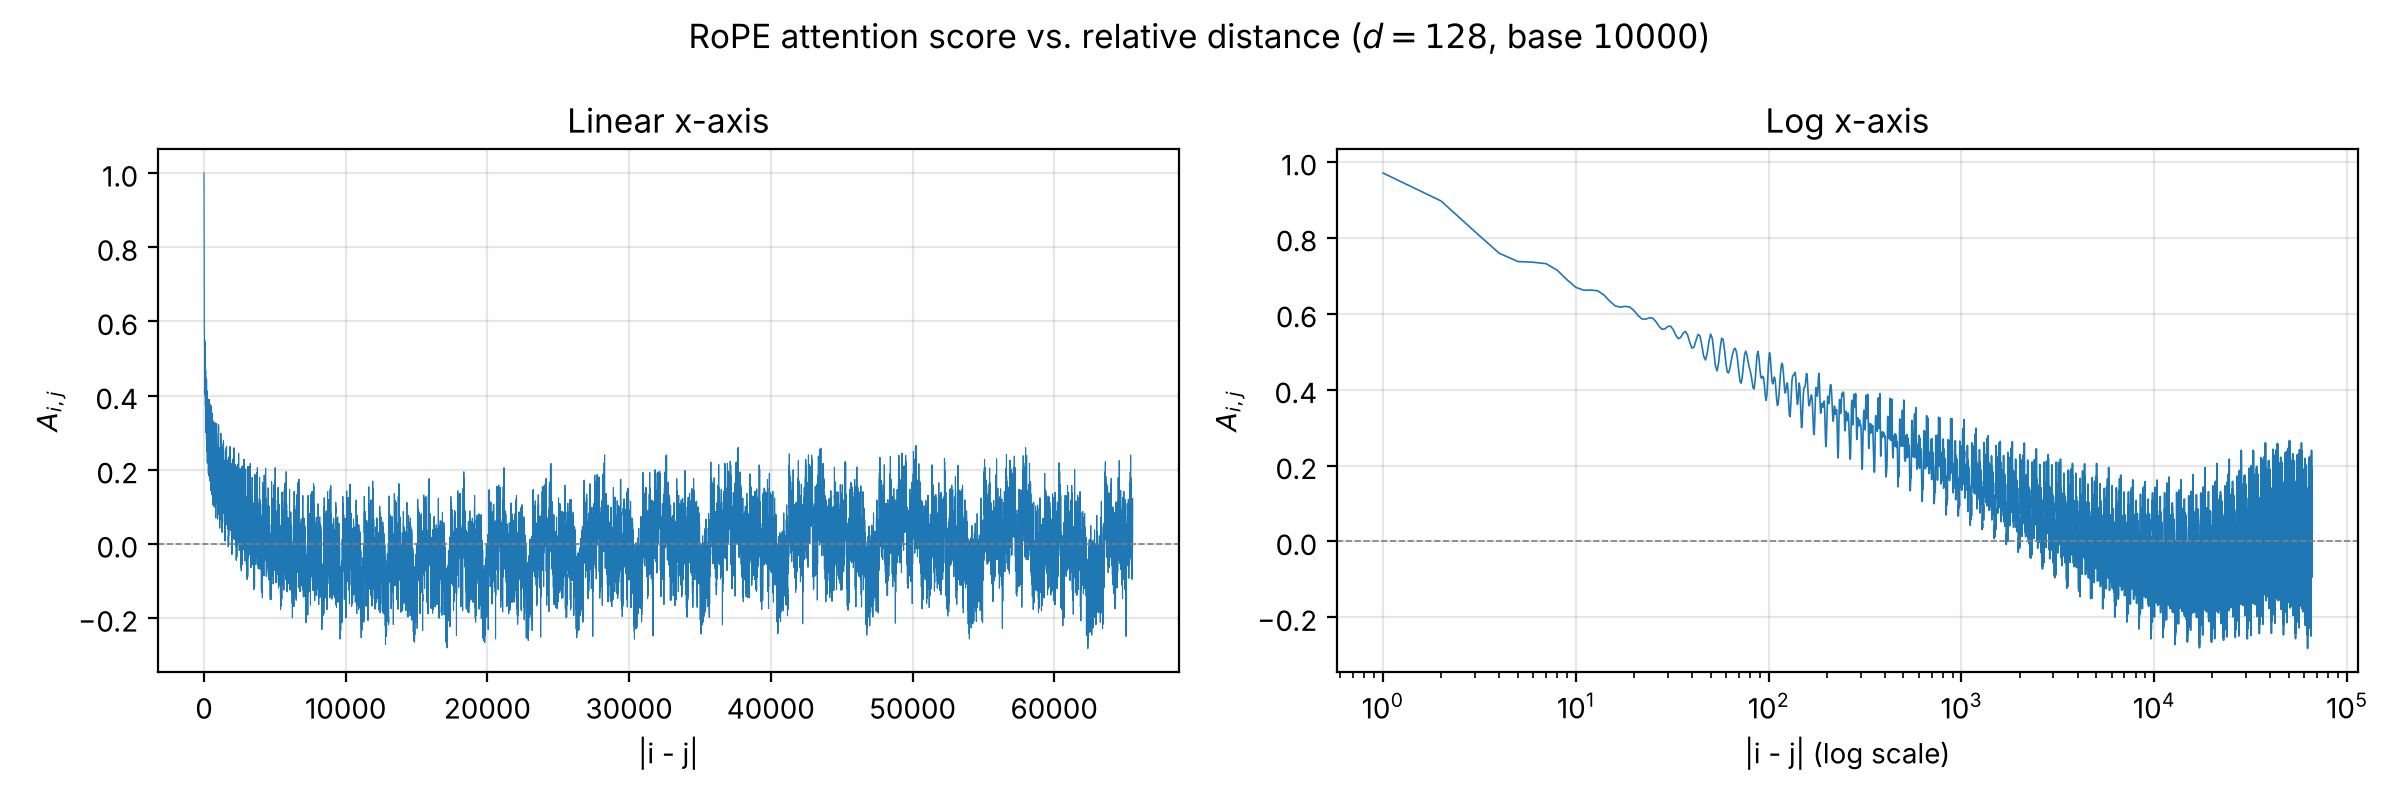
\includegraphics[width=\linewidth]{rope_decay.png}
\end{center}
Produced by \texttt{rope\_plot.py} in the repository. Key values: $A=1$ at $|i-j|=0$, $0.97$ at 1, $0.67$ at 10, $0.48$ at 100, $0.16$ at 1000, and $-0.03$ at $10^4$. The score first drops below $0.5$ at $|i-j|=46$ and first becomes negative at $|i-j|=1707$; beyond $\sim\!4000$ it oscillates around 0 with amplitude up to $\approx\!0.28$ (minimum $-0.28$ at $|i-j|=62376$).

\subsection*{2.3 Limitations suggested by the plot and mitigations}

\textbf{Limitations.}
\begin{itemize}[leftmargin=1.5em]
\item \emph{Long-term decay / recency bias.} Even when content is identical, the prior strongly favors nearby tokens: the score halves within $\sim$50 tokens. Distant tokens must overcome this prior through content similarity, which makes long-range retrieval harder.
\item \emph{No usable positional signal at long range.} Beyond a few thousand tokens the score no longer decays monotonically; it oscillates around zero, so a far-away token can receive a \emph{higher} score than a closer one. Relative order among distant tokens is effectively lost.
\item \emph{Poor length extrapolation.} The wavelengths $2\pi/\theta_t$ range from $\approx 6$ to $\approx 54{,}000$ tokens. If the model is trained on a context much shorter than the slowest wavelengths, the low-frequency dimensions never see a full range of rotation angles during training. At inference beyond the training length those dimensions take angle values that are out of distribution, and perplexity blows up. The effective context window is therefore tied to the training length.
\end{itemize}

\textbf{Mitigations.}
\begin{itemize}[leftmargin=1.5em]
\item \emph{Position Interpolation (PI):} rescale positions $m\mapsto m\cdot L_{\text{train}}/L_{\text{target}}$ so that all angles stay within the trained range, followed by a short fine-tune.
\item \emph{Frequency rescaling:} NTK-aware scaling, YaRN and LongRoPE rescale the base or individual frequencies (interpolating low frequencies, keeping high frequencies) and YaRN also adjusts the attention temperature.
\item \emph{Larger RoPE base:} e.g.\ Llama~3 uses base $500{,}000$, which slows rotation so long distances remain distinguishable.
\item \emph{Continued pre-training on long sequences} after adjusting RoPE (progressive context extension).
\item \emph{Alternative or complementary schemes:} ALiBi (linear distance bias with better extrapolation), sliding-window attention, attention sinks, or partial RoPE (applying RoPE to only a subset of dimensions).
\end{itemize}

%======================================================================
\section*{Problem 3: Model Architecture for Grammar Error Correction}

\subsection*{3.1 Architecture}

GEC is a monolingual sequence-to-sequence task (``translate'' an erroneous sentence into a corrected one), so I use a Transformer \textbf{encoder--decoder}, initialized from a pretrained denoising seq2seq model (e.g.\ BART-base or T5-base).

\begin{center}
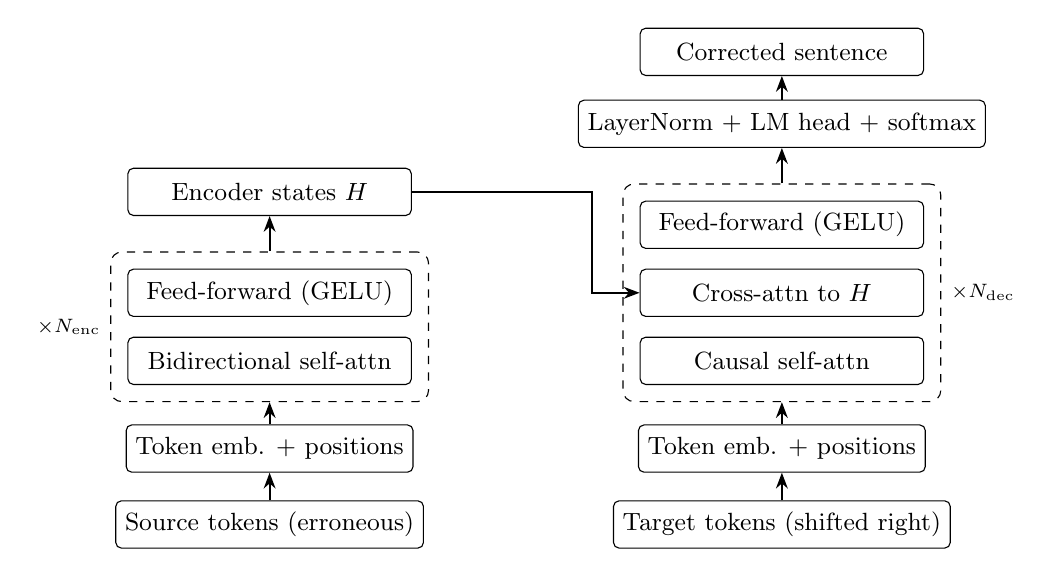
\begin{tikzpicture}[
  font=\small,
  blk/.style={draw, rounded corners=2pt, minimum width=3.6cm, minimum height=0.6cm, align=center, fill=white},
  arr/.style={-{Stealth[length=2mm]}, thick}]
% encoder
\node[blk] (ein) {Source tokens (erroneous)};
\node[blk, above=0.35cm of ein] (eemb) {Token emb. + positions};
\node[blk, above=0.5cm of eemb] (esa) {Bidirectional self-attn};
\node[blk, above=0.25cm of esa] (effn) {Feed-forward (GELU)};
\node[draw, dashed, rounded corners, fit=(esa)(effn), inner sep=6pt, label={[font=\scriptsize]left:$\times N_{\text{enc}}$}] (ebox) {};
\node[blk, above=0.45cm of ebox] (eout) {Encoder states $H$};
% decoder
\node[blk, right=2.4cm of ein] (din) {Target tokens (shifted right)};
\node[blk, above=0.35cm of din] (demb) {Token emb. + positions};
\node[blk, above=0.5cm of demb] (dsa) {Causal self-attn};
\node[blk, above=0.25cm of dsa] (dca) {Cross-attn to $H$};
\node[blk, above=0.25cm of dca] (dffn) {Feed-forward (GELU)};
\node[draw, dashed, rounded corners, fit=(dsa)(dca)(dffn), inner sep=6pt, label={[font=\scriptsize]right:$\times N_{\text{dec}}$}] (dbox) {};
\node[blk, above=0.45cm of dbox] (head) {LayerNorm + LM head + softmax};
\node[blk, above=0.3cm of head] (dout) {Corrected sentence};
% arrows
\draw[arr] (ein) -- (eemb); \draw[arr] (eemb) -- (ebox); \draw[arr] (ebox) -- (eout);
\draw[arr] (din) -- (demb); \draw[arr] (demb) -- (dbox); \draw[arr] (dbox) -- (head); \draw[arr] (head) -- (dout);
\draw[arr] (eout.east) -| ([xshift=-0.6cm]dca.west) -- (dca.west);
\end{tikzpicture}
\end{center}

\textbf{Building blocks} (BART-base--sized configuration):
\begin{itemize}[leftmargin=1.5em]
\item \textbf{Tokenizer:} subword BPE/SentencePiece with $\sim$32k--50k vocabulary, which handles misspellings gracefully by splitting them into subwords.
\item \textbf{Embeddings:} token embedding ($d_{\text{model}}=768$) plus positional encoding (learned absolute or RoPE), with dropout $0.1$. The input embedding, output embedding and LM head share weights.
\item \textbf{Encoder} ($N_{\text{enc}}=6$--$12$ layers): each layer has bidirectional multi-head self-attention (12 heads, head dim 64) and a position-wise FFN ($768\to3072\to768$, GELU), each wrapped with a residual connection and LayerNorm (pre-LN for training stability). It builds a contextual representation of the whole erroneous sentence, which is needed because many errors (agreement, tense) depend on both left and right context.
\item \textbf{Decoder} ($N_{\text{dec}}=6$--$12$ layers): causal (masked) self-attention over the tokens generated so far; cross-attention whose queries come from the decoder and keys/values from the encoder output $H$, which lets the decoder look up and copy source tokens; then an FFN, all with residuals and LayerNorm.
\item \textbf{Output layer:} final LayerNorm, linear projection to the vocabulary (tied weights), and softmax giving $p(y_t\mid y_{<t},x)$.
\item \textbf{Optional copy mechanism:} since most output tokens are copied unchanged from the input, a pointer--generator gate $p_{\text{gen}}$ can mix the vocabulary distribution with the cross-attention distribution over source tokens.
\end{itemize}
\emph{Alternatives:} a decoder-only LLM prompted or fine-tuned with ``Correct: \texttt{<src>} $\Rightarrow$ \texttt{<tgt>}'', or a sequence-tagging model (GECToR: encoder + per-token edit tags such as KEEP / DELETE / APPEND\_$w$ / REPLACE\_$w$), which is several times faster at inference because it is non-autoregressive.

\subsection*{3.2 Input, output and training}

\textbf{Input:} a possibly ungrammatical sentence or paragraph, tokenized into subwords (max length $\sim$128--256 tokens). \textbf{Output:} the corrected text, generated autoregressively; edits are extracted afterwards by aligning source and output (e.g.\ with ERRANT).

\textbf{Data (three stages).}
\begin{enumerate}[leftmargin=1.5em]
\item \emph{Synthetic pre-training:} tens of millions of (corrupted, clean) pairs created by injecting realistic noise into clean text, such as token deletion/insertion/substitution/swap, confusion sets (their/there, a/an), verb-form and agreement errors, and character-level typos. Back-translation (a clean$\to$noisy model) can produce more natural errors.
\item \emph{Fine-tuning on real learner data:} Lang-8, NUCLE, FCE, and W\&I+LOCNESS train.
\item \emph{Final fine-tuning} on the highest-quality in-domain data (W\&I+LOCNESS) with a lower learning rate.
\end{enumerate}

\textbf{Loss.} Token-level cross-entropy with teacher forcing,
\[
\mathcal{L}=-\frac{1}{|y|}\sum_{t=1}^{|y|}\log p_\theta(y_t\mid y_{<t},x),
\]
with label smoothing $\epsilon=0.1$. Correct sentences are kept as identity pairs ($\sim$10--20\% of the data) so the model learns not to over-correct.

\textbf{Optimization and hyper-parameters.}
\begin{center}
\begin{tabular}{@{}p{3.2cm}p{6.6cm}p{4.4cm}@{}}
\toprule
 & Synthetic pre-training & Fine-tuning \\
\midrule
Optimizer & AdamW, $\beta=(0.9,0.98)$, $\epsilon=10^{-8}$, wd $0.01$ & same \\
Peak learning rate & $3\times10^{-4}$ (from scratch) / $1\times10^{-4}$ (from BART) & $3\times10^{-5}$ \\
Schedule & linear warm-up 4k steps, then inverse-sqrt or cosine decay & warm-up 500 steps, linear decay \\
Batch size & $\sim$64k tokens per step & $\sim$16k tokens per step \\
Iterations & $\sim$100k--200k steps & $\sim$5k--10k steps (a few epochs) \\
Regularization & dropout 0.1, label smoothing 0.1, grad-clip 1.0 & dropout 0.1--0.3 \\
Precision & bf16 mixed precision & bf16 \\
\bottomrule
\end{tabular}
\end{center}
Checkpoints are selected by early stopping on the BEA-2019 dev set.

\textbf{Inference and evaluation.} Beam search (beam 5) with a length penalty; optionally iterative decoding (re-feed the output until it no longer changes) and a confidence threshold that favors copying, to improve precision. Evaluation uses the ERRANT $F_{0.5}$ score on BEA-2019 and the $M^2$ $F_{0.5}$ score on CoNLL-2014. $F_{0.5}$ weights precision twice as much as recall, because a wrong ``correction'' hurts the user more than a missed one.

%======================================================================
\newcommand{\fig}[2]{%
  \IfFileExists{#1}{\includegraphics[width=#2\linewidth]{#1}}%
  {\fbox{\parbox[c][4cm][c]{#2\linewidth}{\centering\texttt{\detokenize{#1}}\\(place the image next to this .tex file)}}}}

\section*{Problem 4: Mini-LLM Exercise (nanoGPT)}

\textbf{Setup.} All runs use nanoGPT's \texttt{config/train\_shakespeare\_char.py}: a character-level model with 6 layers, 6 heads, $d_{\text{model}}=384$, context length 256, dropout 0.2, batch size 64, AdamW, cosine decay to \texttt{min\_lr}$=$\texttt{lr}/10, \textbf{5000 iterations}, and the \textbf{fixed seed 1337}. Training was done on a single RTX 5090 (\texttt{compile=False}, bf16). Each variant changes \emph{exactly one} component relative to the baseline and is selected by a command-line switch (\texttt{--norm\_type}, \texttt{--mlp\_type}, \texttt{--pos\_type}, \texttt{--n\_kv\_head}). The exact commands are in \texttt{run\_experiments.ps1} in the repository.

\textbf{Metric.} The dataset is small and every model overfits after about 1500--2500 iterations, so I report the \emph{best validation loss} reached during training (nanoGPT only saves a checkpoint when the validation loss improves).

\textbf{Run-to-run noise.} The original, unmodified code (\texttt{baseline}) reached 1.4751, while the modified code with all switches at their default values (\texttt{baseline2}, which is architecturally identical) reached 1.4632 with the same seed. The difference comes from non-deterministic CUDA kernels. Differences below $\approx 0.01$--$0.015$ should therefore be treated as noise. All comparisons below use \texttt{baseline2}, because it shares the code path with the variants.

\textbf{Learning-rate tuning.} As allowed, I tuned the learning rate. Every model was trained with the default $\text{lr}=10^{-3}$ and also with $5\times10^{-4}$ and $2\times10^{-3}$; nothing else was changed. Table~\ref{tab:results} reports both the default-lr number and the best number.

\begin{table}[h]
\centering
\small
\begin{tabular}{@{}lccccc@{}}
\toprule
 & & \multicolumn{2}{c}{Default lr $=10^{-3}$} & \multicolumn{2}{c}{Best over 3 learning rates} \\
\cmidrule(lr){3-4}\cmidrule(lr){5-6}
Model & Params & Val loss & $\Delta$ & Val loss (lr) & $\Delta$ \\
\midrule
Baseline (original code)            & 10.65M & 1.4751 & ---      & ---                      & --- \\
Baseline (modified code, default)   & 10.65M & 1.4632 & 0        & 1.4619 ($2\!\times\!10^{-3}$) & 0 \\
RMSNorm (Q4.2)                      & 10.65M & 1.4662 & $+0.003$ & 1.4585 ($2\!\times\!10^{-3}$) & $-0.003$ \\
SwiGLU (Q4.3)                       & 10.65M & 1.4910 & $+0.028$ & 1.4887 ($2\!\times\!10^{-3}$) & $+0.027$ \\
NoPE (Q4.4)                         & 10.65M & 1.5268 & $+0.064$ & 1.5114 ($5\!\times\!10^{-4}$) & $+0.050$ \\
RoPE (Q4.4)                         & 10.65M & 1.4724 & $+0.009$ & \textbf{1.4565} ($5\!\times\!10^{-4}$) & $-0.005$ \\
GQA, group size 2 (Q4.5)            & 9.76M  & 1.4690 & $+0.006$ & 1.4607 ($2\!\times\!10^{-3}$) & $-0.001$ \\
\bottomrule
\end{tabular}
\caption{Best validation loss (5000 iterations, seed 1337). $\Delta$ is relative to the baseline with the modified code (default lr in columns 3--4, the baseline's own best lr in columns 5--6). Parameter counts are as printed by nanoGPT, which excludes the position-embedding table.}
\label{tab:results}
\end{table}

\begin{table}[h]
\centering
\begin{tabular}{@{}lccc@{}}
\toprule
Model & lr $=5\times10^{-4}$ & lr $=10^{-3}$ & lr $=2\times10^{-3}$ \\
\midrule
Baseline (modified code) & 1.4769 & 1.4632 & 1.4619 \\
RMSNorm & 1.4712 & 1.4662 & 1.4585 \\
SwiGLU  & 1.4926 & 1.4910 & 1.4887 \\
NoPE    & 1.5114 & 1.5268 & 1.5339 \\
RoPE    & 1.4565 & 1.4724 & 1.4652 \\
GQA     & 1.4755 & 1.4690 & 1.4607 \\
\bottomrule
\end{tabular}
\caption{Full learning-rate sweep (best validation loss).}
\label{tab:sweep}
\end{table}

\subsection*{4.1 Baseline}
\begin{center}\fig{fig_baseline.png}{0.75}\end{center}
The baseline reaches its best validation loss of \textbf{1.4751 at iteration 1750}. After that the training loss keeps falling (to 0.62 at iteration 5000) while the validation loss rises to 1.70: the 10.65M-parameter model memorizes the 1M-character training set and overfits clearly in the second half of training.

\subsection*{4.2 Effect of LayerNorm}
\textbf{Pre-LN or post-LN?} nanoGPT uses \textbf{pre-LayerNorm}: in \texttt{Block.forward}, the normalization is applied \emph{inside} the residual branch before each sub-layer,
\[
x \leftarrow x+\operatorname{Attn}(\operatorname{LN}_1(x)),\qquad x\leftarrow x+\operatorname{MLP}(\operatorname{LN}_2(x)),
\]
with an extra final LayerNorm \texttt{ln\_f} before the LM head.

\textbf{Change.} All three LayerNorms (\texttt{ln\_1}, \texttt{ln\_2}, \texttt{ln\_f}) were replaced by
$\operatorname{RMSNorm}(x)=\dfrac{x}{\sqrt{\frac{1}{d}\sum_i x_i^2+\epsilon}}\odot g$,
which drops the mean subtraction (and the bias, which nanoGPT already disables), so the parameter count is unchanged.

\begin{center}\fig{cmp_rmsnorm.png}{0.75}\end{center}

\textbf{Result.} RMSNorm gives essentially the same loss as LayerNorm: $+0.003$ at the default lr and $-0.003$ after tuning, both within run-to-run noise. This matches the motivation for RMSNorm: re-centering contributes little, while the re-scaling invariance does the work. RMSNorm is slightly cheaper, needing one reduction instead of two, which is why modern LLMs (Llama, Mistral, etc.) use it.

\subsection*{4.3 Effect of MLP}
\textbf{Original activation:} \textbf{GELU}, with $\operatorname{MLP}(x)=W_2\,\operatorname{GELU}(W_1x)$ and hidden size $4d=1536$.

\textbf{Change.} SwiGLU: $\operatorname{MLP}(x)=W_2\big(\operatorname{SiLU}(W_1x)\odot W_3x\big)$. To keep the parameter count the same, the hidden size is set to $\tfrac{8}{3}d=1024$: $3\cdot384\cdot1024=2\cdot384\cdot1536=1{,}179{,}648$ parameters per layer, so the total stays 10.65M exactly.

\begin{center}\fig{cmp_swiglu.png}{0.75}\end{center}

\textbf{Result.} SwiGLU is slightly but \emph{consistently} worse: $+0.016$ to $+0.028$ at every learning rate (Table~\ref{tab:sweep}), which is larger than the noise level. Its validation loss also peaks earlier (iteration 1500 vs.\ 1750), i.e.\ it overfits sooner. SwiGLU's multiplicative gating makes the MLP more expressive per parameter; in large-scale LLM pre-training, which is data-rich and underfitting, this improves loss. In this tiny, data-poor, overfitting-dominated setting, the extra capacity mostly speeds up memorization, so the benefit does not show up. A larger dataset or stronger regularization would be needed to see SwiGLU's advantage.

\subsection*{4.4 Effect of positional encoding}
\textbf{Original:} \textbf{learned absolute position embeddings}, a table \texttt{wpe} $\in\mathbb{R}^{256\times384}$ added to the token embeddings at the input.

\textbf{Variants.}
\begin{itemize}[leftmargin=1.5em]
\item \textbf{NoPE:} the position embedding is no longer added; the input is just the token embedding.
\item \textbf{RoPE:} no input position embedding; instead, inside every attention layer, the query and key vectors of each head ($d_h=64$) are rotated pairwise by angle $m\theta_t$ with $\theta_t=10000^{-2t/d_h}$ (Problem 2), so $q_m^{\top}k_n$ depends only on $m-n$. RoPE has no learned parameters.
\end{itemize}

\begin{center}\fig{cmp_pos.png}{0.75}\end{center}

\textbf{Results.}
\begin{itemize}[leftmargin=1.5em]
\item \textbf{NoPE is clearly worse} at every learning rate ($+0.035$ to $+0.072$; best 1.5114 vs.\ 1.4619). It still learns a reasonable model, because a causal decoder can infer position implicitly: token $m$ attends over exactly $m$ tokens, so the model can ``count''. But this implicit signal is weaker than explicit positions, which matter a lot for character-level modeling (spelling, word boundaries, line structure).
\item \textbf{RoPE matches or slightly beats the learned embedding}. It reached the best number of all runs, 1.4565 at lr $5\times10^{-4}$ ($-0.005$ vs.\ the tuned baseline, and $-0.020$ vs.\ the baseline at the same lr), but the gain over the best baseline is within noise. RoPE injects \emph{relative} position directly into every attention score in every layer, without learning a table, and preferred a lower learning rate here.
\end{itemize}

\subsection*{4.5 Effect of GQA}
\textbf{Change.} The 6 query heads now share 3 key/value heads (group size 2: query heads $\{0,1\}$ use KV head 0, $\{2,3\}$ use KV head 1, $\{4,5\}$ use KV head 2). The fused \texttt{c\_attn} projection outputs $(6+2\cdot3)\cdot64=768$ instead of $1152$ dimensions, and K/V are expanded with \texttt{repeat\_interleave} before attention. This removes $6\times384\times384\approx0.88$M parameters (10.65M $\to$ 9.76M).

\begin{center}\fig{cmp_gqa.png}{0.75}\end{center}

\textbf{Result.} GQA matches the baseline: $+0.006$ at the default lr and $-0.001$ after tuning, both within noise, while using 8\% fewer parameters. Its main benefit appears at inference time: the KV cache is \textbf{halved}, which reduces memory and bandwidth during autoregressive decoding. That is why GQA is standard in modern LLMs (Llama 2/3, Mistral). With such a short context (256) and small model, the reduced K/V capacity costs no measurable quality.

\subsection*{Summary}
Within the noise level of this setup ($\approx0.01$): RMSNorm and GQA are ``free'' changes (same quality; cheaper normalization and a half-size KV cache); RoPE is as good as or slightly better than learned absolute embeddings; removing positional information (NoPE) clearly hurts; and SwiGLU slightly hurts in this small, overfitting-dominated regime. A more decisive comparison would average several seeds per configuration.

\end{document}
